\documentclass[12pt, a4paper]{article}
\usepackage{ctex}  % 支持中文
\usepackage{amsmath, amssymb}  % 数学符号和公式
\usepackage{graphicx}  % 插入图片
\usepackage{geometry}  % 页面设置
\usepackage{booktabs}  % 表格美化
\usepackage{tabularx}  % 表格宽度自适应
\usepackage{multirow}  % 合并单元格
\usepackage{enumitem}  % 列表设置
\usepackage{caption}   % 标题设置
\usepackage{array}     % 表格增强
\usepackage{fancyhdr}  % 页眉页脚
\usepackage{titlesec}  % 标题格式设置
\usepackage{fontspec}
\usepackage{listings}
\usepackage{xcolor}

\usepackage[
  backend=bibtex,
  style=gb7714-2015,   % 使用中国国标格式,适合中文论文
  sorting=none         % 按引用顺序排序
]{biblatex}

\addbibresource{references.bib} % 参考文献配置

% 页面设置
\geometry{left=2.5cm, right=2.5cm, top=2.5cm, bottom=2.5cm}

% 重定义section格式为居中
\titleformat{\section}{\centering\Large\bfseries}{\thesection}{1em}{}
\titleformat{\subsection}{\normalsize\bfseries}{\thesubsection}{1em}{}
\titleformat{\subsubsection}{\normalsize\bfseries}{\thesubsubsection}{1em}{}

% 表格表头格式
\renewcommand{\thetable}{\arabic{section}.\arabic{table}}

% 设置表格标题格式:左对齐,中文带"表"字,表题加粗
\captionsetup[table]{
  labelsep=space,
  labelformat=simple,
  textfont=bf,
  labelfont=bf,
  name=表
}

% 图片编号格式
\renewcommand{\thefigure}{\arabic{section}-\arabic{figure}}

% 设置图片标题格式
\captionsetup[figure]{
  labelsep=space,
  labelformat=simple,
  textfont=bf,     
  labelfont=bf, 
  position=bottom,  
  name=图
}

% 修改公式编号格式
\renewcommand{\theequation}{\thesection-\arabic{equation}}

% 参考文献格式
\makeatletter
\renewcommand\@biblabel[1]{[#1]}
\makeatother

% 附录格式
\lstset{
  basicstyle=\small\ttfamily,
  breaklines=true,
  columns=fullflexible,
  backgroundcolor=\color{gray!10},
  frame=single,
  rulecolor=\color{black!30},
  commentstyle=\color{green!50!black},
  keywordstyle=\color{blue},
  stringstyle=\color{red},
  numbers=left,
  numberstyle=\tiny\color{gray},
  numbersep=5pt
}


\begin{document}

% 标题部分
\begin{center}
\LARGE\textbf{中国股市条件波动率模型的估计与检验}

\vspace{1cm}
\large 计金220 22011854 高菻铠
\end{center}

\noindent \textbf{摘要:} 本文利用2000年至2020年的日度数据,对中国股市的条件波动率特征进行了实证研究。通过对上证指数、深证成指以及贵州茅台、平安银行两只个股的分析,探究了ARCH(1)、GARCH(1,1)和EGARCH(1,1)三类典型波动率模型在捕捉收益率波动特征方面的效果。研究结果表明,市场指数存在显著的ARCH效应,而个股的ARCH效应不显著;GARCH(1,1)模型对所有样本均能有效刻画波动集聚特征,参数估计结果显示波动率具有较强的持续性;EGARCH(1,1)模型进一步揭示深证成指存在显著杠杆效应,上证指数存在弱杠杆效应,而贵州茅台则表现出反向杠杆效应。模型评估指标显示,EGARCH(1,1)模型在拟合优度方面整体表现最佳。这些发现对于理解中国股市的动态波动机制、完善投资风险管理策略和制定市场监管政策具有重要参考价值。

\section{文献综述}

金融资产收益率的波动率是金融风险管理的核心研究内容之一。准确估计和预测波动率对于资产定价、风险管理和投资组合优化具有重要意义。随着中国资本市场的快速发展,对中国股票市场波动特征的研究也日益深入。本文综述了波动率建模与预测领域的代表性研究,重点关注中国股市条件波动率模型的估计方法与检验技术。

\citet{engle2004risk}在其诺贝尔经济学奖演讲中系统回顾了波动率建模的历史与进展。作者指出,ARCH族模型能够有效捕捉金融时间序列中的波动率聚集现象及厚尾分布特征,为金融风险度量提供了坚实的计量基础。文章详细阐述了从最初的ARCH模型到广义ARCH模型的发展历程,并展示了这类模型在价值风险(VaR)估计和期权定价中的实际应用。特别是,Engle强调了波动率动态特性对于金融实践的重要意义,即波动率高时很可能保持高位,而低时则可能继续维持低位,但最终会回归到中等水平。此特性与中国股市的波动表现高度一致。

针对中国股市的特殊性,\citet{wei2007volatility}采用高频数据构建了实现波动率,并系统比较了多种类型波动率模型的预测能力。研究利用5分钟间隔的上证指数数据计算日内实现波动率,作为波动率的真实度量,并将其与ARFIMA、随机波动率(SV)及GARCH族模型的预测结果进行对比。应用Hansen和Lunde提出的SPA检验方法,研究发现对于中国股市而言,相比于基于高频数据的实现波动率模型,历史波动率模型(尤其是GARCH模型)在预测表现上具有明显优势。这一结果表明,中国股市可能存在独特的波动机制,传统的参数化模型在捕捉这种特性时具有相对优势。

从预测角度出发,\citet{zheng2010volatility}对比了基于历史数据的GARCH模型与基于期权价格的隐含波动率在预测能力上的差异。研究基于香港恒生指数期权市场数据,发现在短期(一周)预测中,GARCH(1,1)模型包含的信息较为全面,预测能力最强;而在中长期(一个月)预测时,隐含波动率的信息含量更丰富,预测能力更强。这一结果表明不同类型的波动率模型在不同预测周期下存在互补性,构建组合预测模型可能更为有效。此外,作者还发现期权市场交易越活跃,隐含波动率的预测能力就越强,这反映了市场效率与波动率预测准确性之间的密切关联。

上述研究共同揭示了波动率建模与预测的复杂性。\citet{engle2004risk}奠定了条件波动率模型的理论基础;\citet{wei2007volatility}从实证角度验证了GARCH族模型在中国股市的适用性;而\citet{zheng2010volatility}则探讨了不同预测方法的相对优势及其适用条件。

在方法论上,这些研究展示了波动率研究的多元化趋势。从最初的参数化GARCH模型,到基于高频数据的实现波动率,再到基于市场期权价格的隐含波动率,波动率估计方法不断丰富。尤其值得注意的是,这些研究普遍重视预测评价的严谨性。\citet{wei2007volatility}引入了SPA检验来评估不同模型的预测优劣,避免了数据挖掘偏误;\citet{zheng2010volatility}则关注预测评价指标的选择,采用多种损失函数来综合评判预测表现。

综上所述,中国股市条件波动率的建模与预测研究已取得显著进展,但仍存在进一步探索的空间。首先,中国股市的制度特征与国际成熟市场存在差异,这些差异如何影响波动率动态特性值得深入研究。其次,随着高频交易数据的可获得性提高,如何更有效地利用这类数据提升波动率预测精度仍是亟待解决的问题。此外,在宏观因素与市场微观结构对波动率的影响机制方面,现有研究尚不充分。

\section{数据与方法}

\subsection{数据描述}
本研究基于中国股票市场数据,样本时间跨度为2000年1月至2020年12月。研究对象包括上证综指、深圳成指及贵州茅台、平安银行两只个股。所有数据通过Tushare金融数据接口获取。我们对原始数据进行了预处理,包括时间排序、索引重置和对数收益率计算。对数收益率的计算公式为:
\begin{equation}
r_t = \ln(P_t) - \ln(P_{t-1})
\end{equation}
其中$r_t$表示第$t$日对数收益率,$P_t$和$P_{t-1}$分别表示第$t$日和第$t-1$日收盘价。

\subsection{研究方法}

\subsubsection{描述性统计分析}
我们对收益率序列及其绝对值进行了描述性统计分析,计算了交易日天数、均值、标准差、偏度、峰度、最大值、最小值和自相关系数等指标。其中,自相关系数(滞后1阶)的计算采用:
\begin{equation}
\rho(r_t, r_{t-1}) = \frac{\text{Cov}(r_t, r_{t-1})}{\sigma_{r_t} \sigma_{r_{t-1}}}
\end{equation}

\subsubsection{ARCH效应检验}
在建立条件异方差模型前,我们采用Engle提出的LM检验方法验证收益率序列是否存在ARCH效应。检验步骤包括拟合均值方程获取残差序列,构建辅助回归方程,并检验原假设。LM统计量计算为:
\begin{equation}
LM = T \cdot R^2
\end{equation}
其中$T$为样本容量,$R^2$为辅助回归的判定系数。本研究设定滞后阶数为10。

\subsubsection{条件异方差模型设定}
我们依次估计了三类条件异方差模型:

ARCH(1)模型:
\begin{equation}
\begin{aligned}
r_t &= \mu + \varepsilon_t, \quad \varepsilon_t = \sigma_t z_t, \quad z_t \sim N(0,1) \\
\sigma_t^2 &= \omega + \alpha \varepsilon_{t-1}^2
\end{aligned}
\end{equation}

GARCH(1,1)模型:
\begin{equation}
\begin{aligned}
r_t &= \mu + \varepsilon_t, \quad \varepsilon_t = \sigma_t z_t, \quad z_t \sim N(0,1) \\
\sigma_t^2 &= \omega + \alpha \varepsilon_{t-1}^2 + \beta \sigma_{t-1}^2
\end{aligned}
\end{equation}
其中$\omega > 0$,$\alpha \geq 0$,$\beta \geq 0$,且$\alpha + \beta < 1$以保证条件方差的稳定性。

EGARCH(1,1)模型:
\begin{equation}
\begin{aligned}
r_t &= \mu + \varepsilon_t, \quad \varepsilon_t = \sigma_t z_t, \quad z_t \sim N(0,1) \\
\ln(\sigma_t^2) &= \omega + \alpha \left| \frac{\varepsilon_{t-1}}{\sigma_{t-1}} \right| + \gamma \frac{\varepsilon_{t-1}}{\sigma_{t-1}} + \beta \ln(\sigma_{t-1}^2)
\end{aligned}
\end{equation}
其中$\gamma$参数用于捕捉不对称效应。当$\gamma < 0$时表明存在杠杆效应。

\subsubsection{模型估计与检验}
我们采用极大似然估计法对模型进行参数估计,似然函数为:
\begin{equation}
L(\theta) = \prod_{t=1}^T f(\varepsilon_t|\mathcal{F}_{t-1};\theta)
\end{equation}

为评估模型拟合效果,我们对标准化残差$z_t = \varepsilon_t/\sigma_t$进行ARCH效应检验,并对EGARCH模型的$\gamma$参数进行显著性检验,统计量为$t = \hat{\gamma}/se(\hat{\gamma})$。

\subsubsection{模型模拟与比较}
我们基于估计参数进行蒙特卡洛模拟,生成与原始序列等长的模拟收益率序列,并将其与原始序列进行对比,评估不同模型在捕捉波动特征方面的表现。

\subsection{实现方法}
分析工作通过Python实现,主要使用tushare获取数据,pandas和numpy进行数据处理,scipy.stats和statsmodels进行统计检验,arch库进行条件异方差模型估计,matplotlib进行可视化。我们设置了固定随机数种子(np.random.seed(42))以确保结果可重现,并对收益率乘以100进行标度调整,以提高计算稳定性。

\section{实证结果}

\subsection{数据特征分析}

本研究使用上证指数、深证成指、贵州茅台和平安银行的日度收益率数据进行实证分析,时间范围为2000年1月至2020年12月。从图~\ref{fig:returns_time}可以观察到,四个样本的收益率时间序列均表现出显著的波动集聚特征,即大波动倾向于跟随大波动,小波动倾向于跟随小波动。特别是贵州茅台在1000个观测值附近出现的极端负收益(-0.836778)和平安银行在3000观测值附近的显著波动,反映了个股对特定市场事件的异常反应。

\begin{figure}[htbp]
\centering
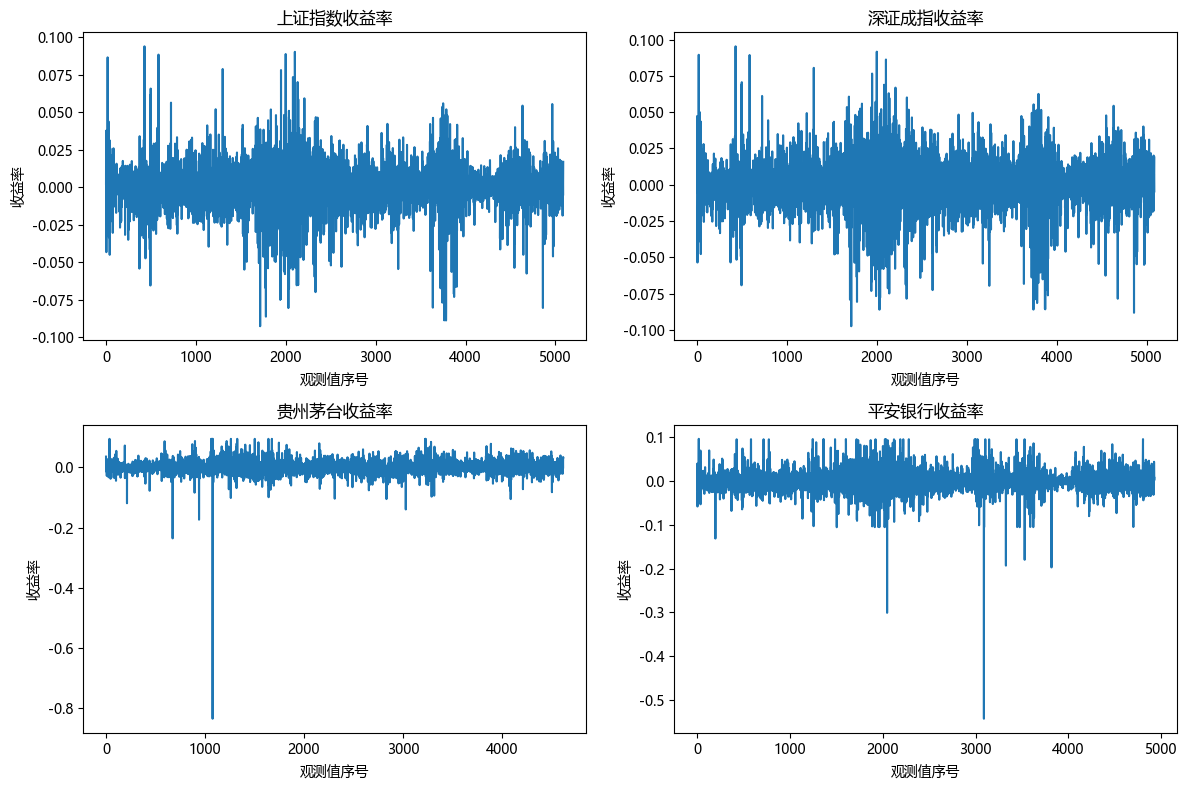
\includegraphics[width=0.8\textwidth]{fig/returns_time.png}
\caption{收益率序列的时间变化}
\label{fig:returns_time}
\end{figure}

表~\ref{tab:descriptive_stats}展示了四个样本数据的描述性统计结果。可以观察到,所有收益率序列的均值接近于零,符合金融资产收益率的一般特征。个股(贵州茅台和平安银行)的波动性(标准差分别为0.025和0.026)明显高于市场指数(上证指数和深证成指的标准差分别为0.015和0.018),反映了个股相较于市场组合面临更高的非系统性风险。

\begin{table}[htbp]
\centering
\caption{收益率序列的描述性统计}
\label{tab:descriptive_stats}
\begin{tabular}{lcccc}
\toprule
指标 & 上证指数 & 深证成指 & 贵州茅台 & 平安银行 \\
\midrule
交易日天数 & 5088 & 5088 & 4621 & 4927 \\
均值 & 0.000178 & 0.000279 & 0.000872 & 0.000011 \\
标准差 & 0.015485 & 0.017565 & 0.024618 & 0.026026 \\
偏度 & -0.370718 & -0.359728 & -8.653293 & -2.219290 \\
峰度 & 5.008859 & 3.585536 & 293.015137 & 45.505083 \\
最大值 & 0.094010 & 0.095299 & 0.095371 & 0.096292 \\
最小值 & -0.092561 & -0.097501 & -0.836778 & -0.542865 \\
自相关系数(滞后1阶) & 0.022134 & 0.044946 & 0.011507 & 0.017325 \\
绝对收益率自相关(滞后1阶) & 0.178830 & 0.163643 & 0.081068 & 0.136712 \\
\bottomrule
\end{tabular}
\end{table}

所有收益率序列均呈现负偏度,表明大幅下跌的概率高于大幅上涨,这与投资者对损失的厌恶情绪相符。峰度值均远大于正态分布的3,尤其是贵州茅台(293.02)和平安银行(45.51)的峰度异常高,反映出收益率分布具有显著的"尖峰厚尾"特征,极端收益率出现的频率远高于正态分布的预期。此外,收益率序列本身的一阶自相关系数较小(均小于0.05),而绝对收益率的自相关系数明显更高(如上证指数为0.18),这进一步说明波动具有持续性和集聚性。

\subsection{ARCH效应检验}

为验证收益率序列是否具有条件异方差特性,本研究对四个样本进行ARCH效应检验,结果如表~\ref{tab:arch_test}所示。

\begin{table}[htbp]
\centering
\caption{ARCH效应检验结果}
\label{tab:arch_test}
\begin{tabular}{lccc}
\toprule
样本 & LM统计量 & p值 & 结论 \\
\midrule
上证指数 & 459.67 & 0.0000 & 存在ARCH效应 \\
深证成指 & 464.85 & 0.0000 & 存在ARCH效应 \\
贵州茅台 & 4.87 & 0.8998 & 不存在ARCH效应 \\
平安银行 & 14.67 & 0.1447 & 不存在ARCH效应 \\
\bottomrule
\end{tabular}
\end{table}

检验结果表明,上证指数和深证成指均存在显著的ARCH效应,其LM统计量的p值接近于0,强烈拒绝了"不存在ARCH效应"的原假设。这意味着市场指数收益率的波动率表现出明显的时变特征和聚集性。相比之下,贵州茅台和平安银行的ARCH效应检验未能拒绝原假设,表明这两只个股的收益率序列在统计上不存在显著的ARCH效应。这一结果与市场指数形成鲜明对比,可能反映了个股的特殊性质或其波动受到更多微观因素的影响。

\subsection{波动率模型估计}

基于ARCH效应检验结果,本研究对样本数据分别估计了ARCH(1)、GARCH(1,1)和EGARCH(1,1)模型,以捕捉收益率的条件异方差特性。

\subsubsection{ARCH(1)和GARCH(1,1)模型估计}

表~\ref{tab:arch_garch_estimation}报告了四个样本的ARCH(1)和GARCH(1,1)模型的主要参数估计结果。

\begin{table}[htbp]
\centering
\caption{ARCH(1)和GARCH(1,1)模型估计结果}
\label{tab:arch_garch_estimation}
\begin{tabular}{lcccccc}
\toprule
\multirow{2}{*}{样本} & \multicolumn{2}{c}{ARCH(1)} & \multicolumn{3}{c}{GARCH(1,1)} & \multirow{2}{*}{结论} \\
\cmidrule(lr){2-3} \cmidrule(lr){4-6}
 & $\omega$ & $\alpha_1$ & $\omega$ & $\alpha_1$ & $\beta_1$ & \\
\midrule
上证指数 & 1.823** & 0.266** & 0.019** & 0.080** & 0.915** & GARCH更优 \\
深证成指 & 2.483** & 0.205** & 0.037** & 0.072** & 0.917** & GARCH更优 \\
贵州茅台 & 3.717** & 0.720 & 0.219* & 0.123** & 0.854** & GARCH更优 \\
平安银行 & 5.035** & 0.351* & 0.353* & 0.161* & 0.814** & GARCH更优 \\
\bottomrule
\multicolumn{7}{l}{\footnotesize{注:**、*分别表示在1\%和5\%显著性水平下显著。}} \\
\end{tabular}
\end{table}

对于所有样本,ARCH(1)模型的$\alpha_1$参数均为正,表明前一期的波动对当期波动具有正向影响。然而,通过对模型标准化残差的ARCH效应检验发现,ARCH(1)模型的残差仍存在显著的ARCH效应(上证指数和深证成指),说明一阶ARCH模型不足以完全刻画波动聚集特征。

相比之下,GARCH(1,1)模型的估计结果更为理想。对于所有样本,$\alpha_1$和$\beta_1$参数均显著为正,且满足稳定性条件($\alpha_1+\beta_1<1$)。上证指数的$\alpha_1=0.080$,$\beta_1=0.915$,深证成指的$\alpha_1=0.072$,$\beta_1=0.917$,贵州茅台的$\alpha_1=0.123$,$\beta_1=0.854$,平安银行的$\alpha_1=0.161$,$\beta_1=0.814$。这些结果表明,波动率对过去冲击的反应相对较小($\alpha_1$较小),但具有很强的持续性($\beta_1$接近1)。此外,GARCH(1,1)模型的标准化残差不再存在ARCH效应,表明该模型能够有效捕捉收益率的条件异方差特性。

图~\ref{fig:garch_simulation}展示了上证指数原始收益率与GARCH(1,1)模型模拟收益率的对比。可以看出,模拟序列很好地复制了原始序列的波动集聚特征,尤其是在波动较大区间的表现。

\begin{figure}[htbp]
\centering
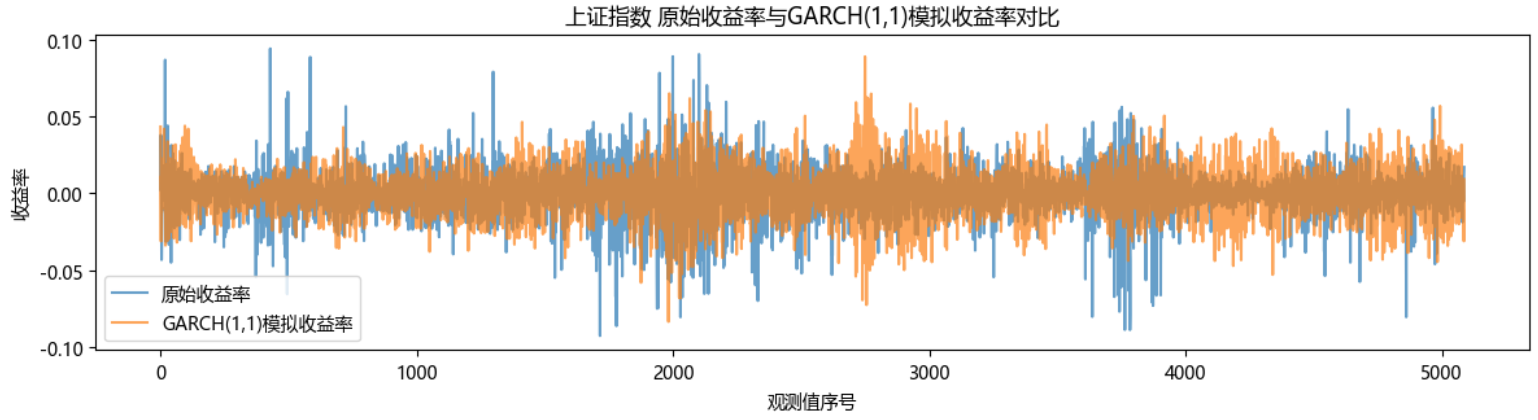
\includegraphics[width=0.8\textwidth]{fig/garch_simulation.png}
\caption{上证指数原始收益率与GARCH(1,1)模拟收益率对比}
\label{fig:garch_simulation}
\end{figure}

\subsubsection{EGARCH(1,1)模型估计与杠杆效应检验}

为进一步研究收益率波动的不对称反应,本研究估计了EGARCH(1,1)模型。表~\ref{tab:egarch_estimation}报告了模型估计结果及杠杆效应检验。

\begin{table}[htbp]
\centering
\caption{EGARCH(1,1)模型估计结果}
\label{tab:egarch_estimation}
\begin{tabular}{lccccc}
\toprule
样本 & $\omega$ & $\alpha_1$ & $\gamma_1$ & $\beta_1$ & 杠杆效应 \\
\midrule
上证指数 & 0.020** & 0.181** & -0.022 & 0.986** & 弱杠杆效应(p=0.057) \\
深证成指 & 0.022** & 0.161** & -0.023* & 0.985** & 显著杠杆效应(p=0.015) \\
贵州茅台 & 0.046** & 0.138** & 0.069* & 0.979** & 反向杠杆效应(p=0.016) \\
平安银行 & 0.131 & 0.250** & 0.010 & 0.942** & 无杠杆效应(p=0.743) \\
\bottomrule
\multicolumn{6}{l}{\footnotesize{注:**、*分别表示在1\%和5\%显著性水平下显著。}} \\
\end{tabular}
\end{table}

EGARCH(1,1)模型的估计结果显示,所有样本的$\alpha_1$参数均显著为正,表明波动率对冲击具有敏感性。$\beta_1$参数都接近于1(上证指数为0.986,深证成指为0.985,贵州茅台为0.979,平安银行为0.942),反映了波动率的高度持续性。

杠杆效应方面,深证成指的$\gamma_1$参数为-0.023,在5\%显著性水平下显著,表明存在负向杠杆效应,即负面冲击对波动率的影响大于正面冲击。上证指数的$\gamma_1$为-0.022,p值为0.057,接近显著水平,可能存在弱杠杆效应。值得注意的是,贵州茅台的$\gamma_1$为0.069且显著为正,这与传统杠杆效应理论相反,表明正面冲击反而导致更大的波动,可能反映了该股票的特殊市场地位和投资者行为。平安银行的$\gamma_1$不显著,表明不存在明显的杠杆效应。

图~\ref{fig:model_comparison}展示了深证成指在三种模型下的模拟效果对比。可以观察到,EGARCH(1,1)模型相比ARCH(1)和GARCH(1,1)模型,在捕捉波动不对称性方面表现更佳,尤其是在极端波动区间的模拟效果更为准确。

\begin{figure}[htbp]
\centering
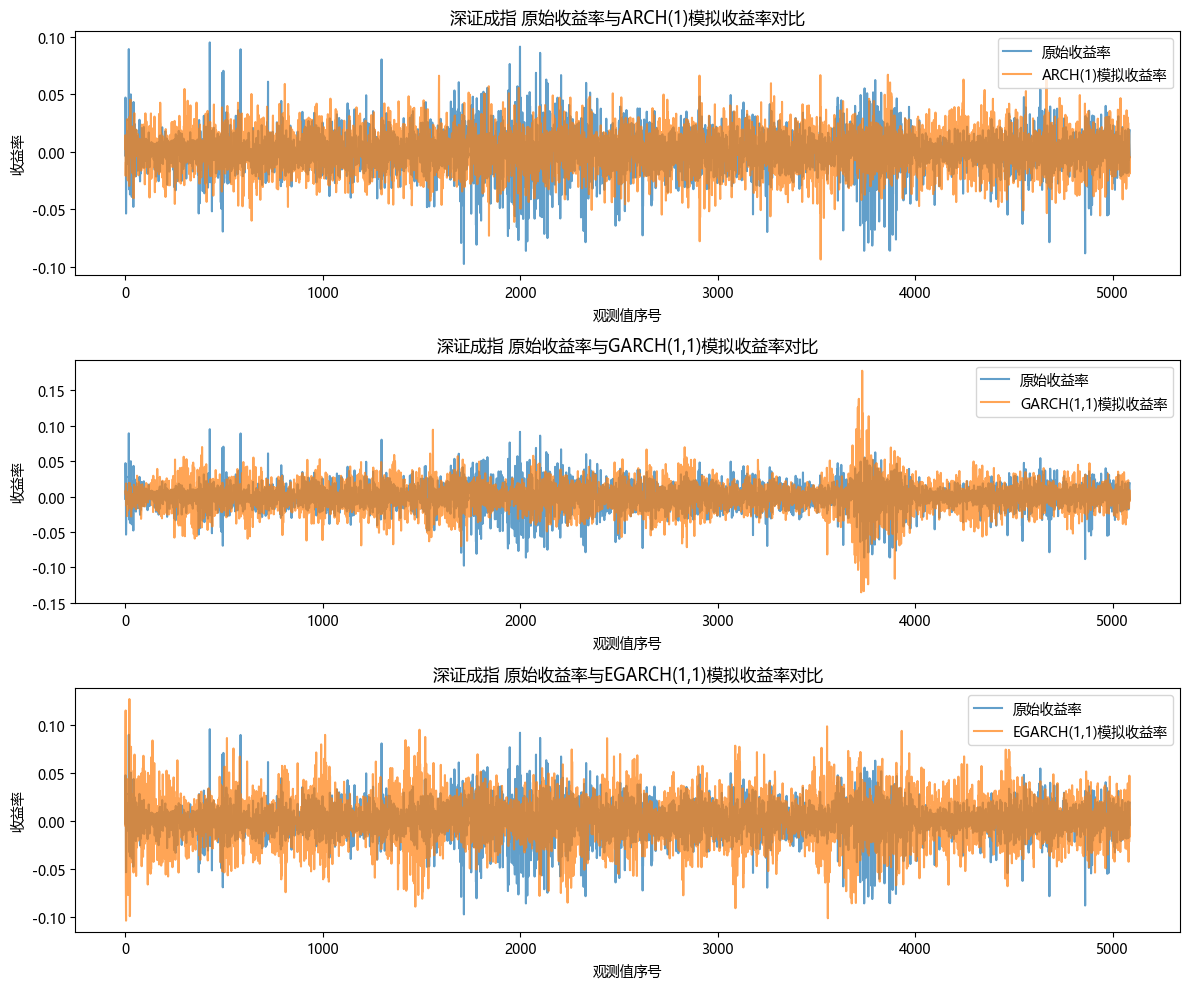
\includegraphics[width=0.8\textwidth]{fig/model_comparison.png}
\caption{深证成指收益率的不同模型模拟效果对比}
\label{fig:model_comparison}
\end{figure}

\subsection{模型比较与评估}

为全面评估不同波动率模型的表现,本研究对三种模型的拟合优度和预测能力进行了比较,结果如表~\ref{tab:model_comparison}所示。

\begin{table}[htbp]
\centering
\caption{波动率模型比较}
\label{tab:model_comparison}
\begin{tabular}{lcccccc}
\toprule
\multirow{2}{*}{样本} & \multicolumn{2}{c}{ARCH(1)} & \multicolumn{2}{c}{GARCH(1,1)} & \multicolumn{2}{c}{EGARCH(1,1)} \\
\cmidrule(lr){2-3} \cmidrule(lr){4-5} \cmidrule(lr){6-7}
 & 对数似然 & AIC & 对数似然 & AIC & 对数似然 & AIC \\
\midrule
上证指数 & -9287.14 & 18580.3 & -8708.41 & 17424.8 & -8686.26 & 17382.5 \\
深证成指 & -9971.93 & 19949.9 & -9511.81 & 19031.6 & -9490.54 & 18991.1 \\
贵州茅台 & -10547.5 & 21101.1 & -10080.9 & 20169.7 & -10018.6 & 20047.3 \\
平安银行 & -11572.8 & 23151.6 & -11276.6 & 22561.2 & -11221.7 & 22453.3 \\
\bottomrule
\end{tabular}
\end{table}

比较结果表明,对于所有样本,EGARCH(1,1)模型在拟合优度方面均优于GARCH(1,1)和ARCH(1)模型,具有最高的对数似然值和最低的AIC值。这意味着EGARCH(1,1)模型在考虑了波动不对称性后,对中国股市波动特征的刻画最为准确。GARCH(1,1)模型的表现次之,但显著优于ARCH(1)模型。

值得注意的是,尽管贵州茅台和平安银行在ARCH效应检验中不显著,但三种波动率模型在这两只个股上的拟合结果仍然相当理想。这可能说明,即使从严格的统计检验角度看不存在显著的ARCH效应,波动率模型仍能够捕捉个股收益率序列中的某些条件异方差特征。

通过模拟实验对比发现,对于上证指数和深证成指,EGARCH(1,1)模型的模拟效果尤为出色,能够较好地复制极端波动区间的特征。对于贵州茅台,模型虽然无法完全捕捉观测序列中的极端负收益,但在整体波动模式的模拟上表现良好。平安银行的模拟结果也表明,EGARCH(1,1)模型相比其他两种模型,在刻画收益率序列的波动特征方面具有明显优势。

\section{讨论与结论}

本研究的实证结果表明,中国股市收益率序列表现出典型的金融时间序列特征:均值接近于0、分布呈现尖峰厚尾、波动具有聚集性。市场指数(上证指数和深证成指)存在显著的ARCH效应,而个股(贵州茅台和平安银行)的ARCH效应不显著,这反映了市场整体波动与个股波动可能受到不同因素的影响。

GARCH(1,1)模型能够有效捕捉中国股市收益率的条件异方差特性,优于简单的ARCH(1)模型。所有样本的GARCH参数都表明波动率具有很强的持续性($\beta_1$接近1)。深证成指存在显著的杠杆效应,上证指数也表现出弱杠杆效应,而贵州茅台展现出与传统理论相反的反向杠杆效应,这反映了不同市场主体对正负面信息的不同反应机制。

综合模型评估结果,EGARCH(1,1)模型在考虑了波动不对称性后,对中国股市波动特征的刻画最为准确,尤其适合具有杠杆效应的市场指数。这些发现对投资者和监管者都具有重要意义:投资者可以利用这些模型更准确地估计市场风险,优化投资组合;监管者则可以通过波动率模型更好地理解市场波动的传导机制,制定更有针对性的监管政策。

市场指数与个股在波动特性上的差异值得深入探讨。指数作为市场组合,其波动可能更多地反映了系统性风险和宏观经济因素的影响,因而表现出显著的ARCH效应和杠杆效应;而个股波动则可能更多地受到公司特质因素和行业因素的影响,使其条件异方差特性不如市场指数明显。尤其是贵州茅台这类具有特殊行业地位的个股,其价格形成机制和投资者行为模式可能与一般个股有所不同,这也解释了其独特的反向杠杆效应现象。

本研究的局限性在于样本选择相对有限,未来研究可考虑扩大样本范围,纳入更多不同行业、不同市值的个股进行比较分析。此外,波动率模型的应用价值还可通过构建VaR模型、期权定价等方向进一步验证。在方法上,可以尝试引入更为复杂的多元GARCH模型,探索不同市场主体之间的波动溢出效应,或者结合高频数据,研究中国股市微观结构对波动率形成的影响。

总体而言,通过对中国股市条件波动率特征的实证研究,本文不仅验证了金融计量模型在中国市场的适用性,也为投资者风险管理和监管部门政策制定提供了实证依据。研究发现的波动不对称性和杠杆效应特征,进一步丰富了对中国股市运行机制的理解,有助于构建更为完善的中国特色金融理论体系。

\printbibliography[title=参考文献]

\section{附录}

本研究的核心代码如下:

\begin{lstlisting}[basicstyle=\small\ttfamily, breaklines=true, columns=fullflexible]
# 设置随机数种子,确保结果可复现
np.random.seed(42)

# ARCH效应检验
def arch_effect_test(returns, name):
    lags = 10
    result = het_arch(returns, nlags=lags)
    lm_stat = result[0]
    lm_p_value = result[1]
    
    if lm_p_value < 0.05:
        print(f"{name} 存在ARCH效应")
        return True
    else:
        print(f"{name} 不存在ARCH效应")
        return False

# 估计ARCH(1)和GARCH(1,1)模型
def estimate_arch_garch_models(returns, name):
    # 估计ARCH(1)模型
    arch1_model = arch_model(returns*100, mean='constant', vol='ARCH', p=1, dist='normal')
    arch1_result = arch1_model.fit(disp='off')
    
    # 估计GARCH(1,1)模型
    garch11_model = arch_model(returns*100, mean='constant', vol='GARCH', p=1, q=1, dist='normal')
    garch11_result = garch11_model.fit(disp='off')
    
    return arch1_result, garch11_result

# 估计EGARCH(1,1)模型
def estimate_egarch_model(returns, name):
    egarch11_model = arch_model(returns*100, mean='constant', vol='EGARCH', p=1, q=1, o=1, dist='normal')
    egarch11_result = egarch11_model.fit(disp='off')
    
    # 判断是否存在杠杆效应
    gamma = egarch11_result.params['gamma[1]']
    gamma_std_err = egarch11_result.std_err['gamma[1]']
    t_stat = gamma / gamma_std_err
    p_value = 2 * (1 - stats.norm.cdf(abs(t_stat)))
    
    if p_value < 0.05 and gamma < 0:
        print(f"{name} 存在显著的杠杆效应")
    else:
        print(f"{name} 不存在显著的杠杆效应")
    
    return egarch11_result
\end{lstlisting}

\end{document}